\part{State of the Art}

\chapter{Optimization}

\section{Basic Concepts}

Before starting to present the different categories of optimization, we would like to take some time defining what exactly optimization is.\\
In the more general way, optimizing is \emph{trying to find the best element among an element set}. When finding this best element is not trivial, we can rightfully talk of \emph{solving an optimization problem}. This seemingly simple definition implies in fact quite a lot.

First of all it requires we have a defined set of element to choose from. As we will see, the topology of the set is of the utmost importance for choosing the way of solving the problem. This set of element is often named the \emph{search space}, \emph{solution space} or \emph{domain}. In "simple" optimization problems, the search space can be simply defined by a set of elements (for example \{a,b,c\} or \ensuremath{\mathbb{R}}) associated with a set of \emph{constraints}. For large problems, the search space can be defined by calculus-heavy equations, empirical models, complex algorithms ... or even a mix of all of the above.

\definition{Search space}{the set containing all the possible candidates of the optimization problem.}

While we said that the search space can be defined by a set of constraints, it is often more convenient to express the constraints separately. For example, if the search space of an optimization problem is defined over all the real numbers lower than 2, instead of defining the search space as [-\(\infty\) : 2], it will usually be refereed as \(\mathbb{R}\), with the added constraint \(x < 2\). Usually we say the problem to be \emph{subject to (s. t.)} the constraint \(x < 2\).\\
In theory these two formulations should be equivalent. In practice however, these constraints are often the result of a real-world concern, and thus subject to some inherent imprecision. [[WHAT ?? THE TRAVEL IS INTRODUCED AFTER]] Back to our travel metaphor, we can imagine that we set the maximum travel cost we are ready pay to a price of one thousand euro. Does that really means that a solution which would cost one thousand euro \textbf{and one cent} would be unacceptable ? Obviously not.  In engineering design, this is a common situation, and making these constraints explicits can be advantageous.

Since we want to find the best element of this solution space, we have to determine what make an element better than another. Usually, the possible solutions are compared through a specific function called the \emph{objective function}. Some alternate names are \emph{criterion} or \emph{cost function}. The best element would be the one for which the objective function returns a minimal (or alternatively, maximal\footnote{Obviously we sometimes want to find the \emph{maximal} value which is solution of a problem, however minimizing f(x) is equivalent to maximizing (-f(x)). So maximization problems can be expressed as minimization problems, and vice-versa. Traditionally, optimization problems are often expressed in the terms of finding a \emph{minimal} value since the two possibilities are equivalents.}) value. It should be noted that it is possible for a problem to admit several equivalent solutions in regard of the objective function.

\definition{Objective function}{a function defined over the search space of the optimization problems.}

The least obvious keyword here is \emph{try}. When the search space is very large, or its topology is complicated, it can be really long or difficult to find the best solution and, more important, to be sure that the solution is the best. In fact, in these problems, the only way to find the best solution with certainty is an exhaustive exploration of the search space. Since it can be very costly in terms
of time and calculation, instead of finding the best solution, we settle for a solution which is "good enough", for example because this solution is the best for a subpart of the search space. The best solution is called the \emph{global optimum}, while a "good enough" solution is called a \emph{local optimum}. In a similar fashion, methods which try to find the global solution are said to be \emph{global optimization methods}, where methods which search for local optimum are said to be \emph{local optimization methods}.

\definition{Optimizing}{finding an element of the search space which minimize (or maximize) the value of the objective-function}


\begin{figure}
\centering
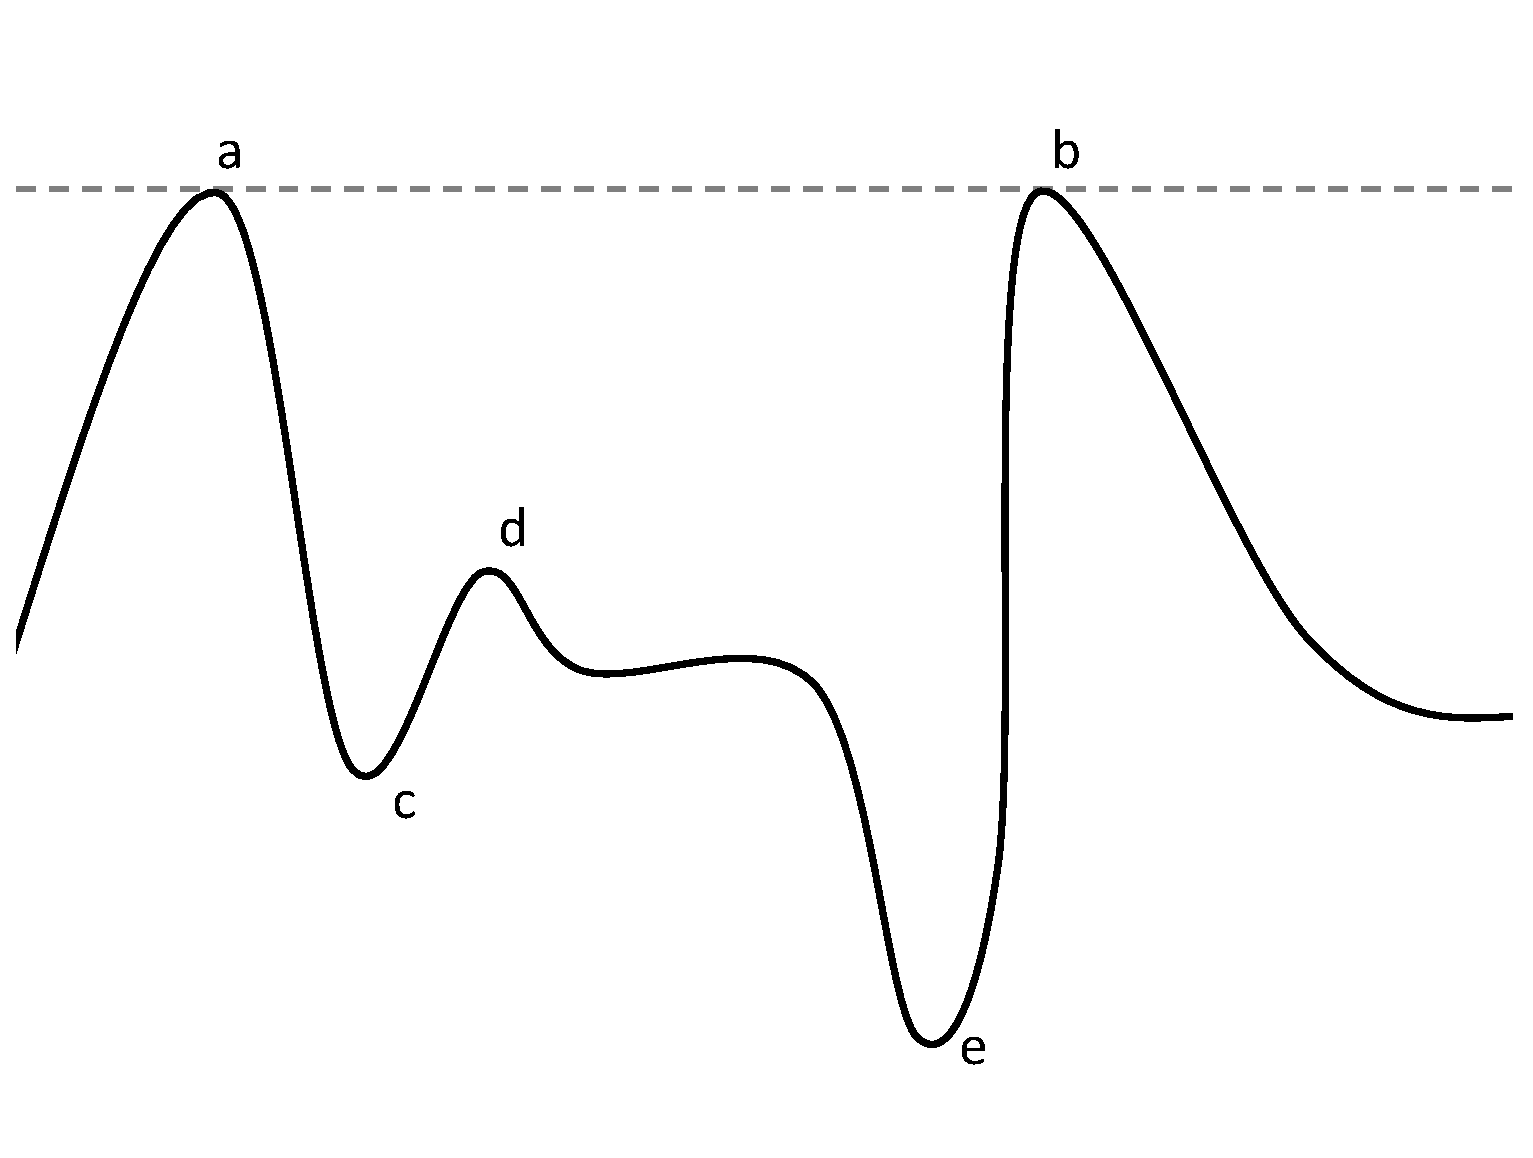
\includegraphics[width=0.6\paperwidth]{searchSpace}
\caption{Examples of local and global optimums.}
\label{localAndGlobalOptims}
\end{figure}

In figure \ref{localAndGlobalOptims}, we can see different examples of global and local optimums. The points labeled \emph{a} and \emph{b} are both global maximums, as they have the same value. The points
\emph{c} and \emph{d} are respectively local minimum and maximum, while \emph{e} is the global minimum.

From all the preceding, we can provide the minimal formulation of an optimization problem as follow 

\definition{Optimization problem}{ [[NOT GOOD]] \(\text{minimize } f(x) \text{ subject to } (x \in S)\)\\
Where \emph{S} is the problem search space and \emph{f(x)} the objective function.}

\subsection{No Free Lunch Theorem}
[[AVANT OU APRES LA DESCRIPTION DES DIFFERENTES METHODES ?]]

[[Compromis entre Exploration et Exploitation cf Berro Thesis]]

\subsection{Combinatorial Optimization}

\section{Numerical Optimization}
\subsection{Linear Programming}
\subsection{Quadratic Programming}
\section{Nonlinear Programming}

\section{Multi-Objective Optimization}

Multi-objective optimization (also called multi-criteria optimization), or MOO, departs significantly from previous categories of optimization in the fact that you have to consider multiple objective functions instead of one. A main aspect of MOO is the way to conciliate these objectives, which are usually contradictory.
An example of real-world everyday MOO problem could be choosing the mean of transportation for a travel, trying to find a balance between speed and cost. Airplane is the fastest way of transportation, but is expensive. While car is slower, it is cheaper. Train is slower than plane, more expensive than car, but can preferred as the best compromise. There still, however, are solutions which are strictly worse than others (in our example, renting an helicopter would probably be both more expensive and slower than buying a seat on a commercial airplane).
From this example we can see that, for a MOO problem, there rarely is a clear-cut "best" solution. And more importantly that even some solutions which are not optimum for \emph{any} of the objectives can be deemed satisfying. Only when each objective is completely independent then a MOO problem can be handled as a set of separated mono-objective optimization problems. 

[[FORMULATION OF A MOO PROBLEM]]

MOO problems are quite a radical departure from previous optimization problems type we have seen. Many approaches have proposed, the majority of which can be separated in to categories: \emph{a priori} and \emph{a posteriori} approaches. A priori approaches aims to discriminate between the objectives \emph{before} the optimization process. This often consist into combining the different objectives into one, before applying a classical optimization method on the new, aggregated objective.
On the opposite, a posteriori methods tries to provide a set of efficient solutions among which the decider will choose.
A priori approaches are considered easier, but not very efficient, whereas a posteriori approaches provides more diversity of solutions as well as more insight about the nature of the problem.
A third category can also be considered: the \emph{interactive} methods. Basically, these methods iterates between decision and search phases. For example, an interactive  method could work by quickly providing intermediate solutions to the decision-maker, which would in return refine the search using them.

We will now see some of the strategies have been proposed to deal with such a type of problem.

\subsection{A Priori Methods - Objectives Aggregation}

The first approach is to transform the MOO problem back to a mono-objective optimization problem, by aggregating the different objectives into one. This can be expressed as follow : \(f_g = aggr(f_1,f_2,...,f_n)\), where \(f_1, f_2...,f_n\) are the original objectives and \(f_g\) the aggregated one, which will be used with classical mono-objective optimization methods. 
Concerning the choice of the aggregation function, different strategies can be used.

\begin{itemize}

\item addition, multiplication, mean, max or min of the objectives: these methods present the major drawback of requiring the aggregated values to be comparable.[[ Keeping with our travel example]], is it relevant to simply add duration and cost ?

\item pondered mean: we attribute a coefficient to each objective when adding them. This method allows to express a preference between different objectives, as well as bringing back on comparable scale different objectives. However, one now has to decide of the coefficients to choose. Also, this method can hide some information concerning the solution, for example an extremely poor result in one of the objectives, compensated by small improvements in all the others.

[[parler de goal programming, min-max etc. ? (cf these berro)]]

\end{itemize}

Whatever the chosen aggregation strategy will be, this approach presents severe limitations.  [[give them]]

\subsection{A Posteriori Methods}

We have seen that, while convenient, \emp{a priori} methods can be quite restrictive. By choosing beforehand a way to aggregate the objectives, we lose in diversity of solutions and influence the result of the optimization process.

\subsubsection{Pareto Dominance}

A radically different approach has be proposed, using the concepts of Pareto dominance and Pareto optimality. These concepts were originally been developed in economical sciences first by Francis Edgeworth and later Vilfredo Pareto. The initial application of the concepts was to propose a minimal definition of "efficiency", regarding allocation of resources inside an economical system.

The main idea is that a state where it is impossible to improve the resources allocation for an individual without worsening the situation of at least another is described as \emph{Pareto efficient}, or \emph{Pareto optimal}.

Conversely, if from a system state A it is possible to find a new state B where at least one individual's situation is improved without worsening the situation of another, the state A will be said to be \emph{Pareto inefficient}. The state B will be said to \emph{dominate} the state A in terms of Pareto optimality, and the passage from A to B will said to be a \emph{Pareto improvement}. This relation of Pareto dominance is usually noted \(\prec\).

\definition{Pareto-dominance}{Given A and B two vectors describing different resources allocations in a system, \(A \prec B \Leftrightarrow (\forall i \text{ }A_i \leq B_i \land \exists j \text{ } A_j < B_j\)). }

Note that in the preceding example, we wanted to maximize resources allocation, so \(A \prec B\) reads " B dominates A". If we want to \emph{minimize} the allocation, the meaning is inverted and  \(A \prec B\) reads "A dominates B".
As it is the standard convention in optimization to express problems in terms of minimization, for the rest of this thesis we will use \(A \prec B\) with the meaning of "A dominates B", unless otherwise specified.

Based on this relation of dominance, it is possible to provide a definition of Pareto-optimality.

\definition{Pareto-optimality}{A solution vector that is dominated no other possible solution is said to be Pareto-optimal.}

\definition{Pareto front}{the set of Pareto-optimal solutions.}

It is also possible to classify the solutions by rank: a solution which is dominated by no other is said to be of rank 0 (and to be Pareto-optimal). A solution which is dominated by at most a solution of rank 0 said to be of rank 1 and so on.

As a remark, these definitions of efficiency and optimality do not give any information about the fairness of the allocation, or the well-being of the involved parties. From this point of view, a monopolistic situation where one actor would control all the available resources is as optimal as a situation where all the resources are equally divided between the individuals.

These definitions of dominance and optimality can be used to characterize the possibles solutions of MOO problem. In this case, the problem is no more to find an optimal solution, but to find the Pareto front of the problem.

[[TODO: give some example of Pareto methods]]
A widespread strategy to find the Pareto front is to use [[population-based]] metaheuristics, such as Multi-Objective Evolutionary Algorithms (MOEA). 

Historically, evolutionary algorithms are divided in two main categories, based on whether or not they use elitism mechanisms, with some consensus concerning the superiority of elitist algorithms.

\subsubsection{Non-elitist evolutionary algorithms}

[[Vector Evaluated Genetic Algorithm (VEGA) Schaffer (1985) => Non Pareto]

[[  Goldberg and Richardson (1987) =>  Simple Pareto domination scheme. • Sharing on whole population]]


\subsubsection{Elitist evolutionary algorithms}

Different possibilities has been explored to introduce elitism in MOAE. A common approach is to use a second population consisting of elite, non-dominated individuals, which are used as recombination partners for the main population.

[[Signal that evolutionary algorithms have difficulties with more than two objectives ?]]

\subsection{Interactive Methods [[?]]}

\section{Multidisciplinary Optimization}

\section{Optimization under Uncertainties}

\section{Optimization in Dynamic Environments}
A special case of optimization is optimization in dynamic environment.

\subsection{Genetic Algorithms}
